\section{预备知识}

\subsection{定义}

\cpar{原生多模态模型 (NMMs):}
从头开始同时训练所有模态的模型,而不依赖于预训练的LLMs或视觉编码器。我们的重点是代表性的图像和文本模态,其中模型处理文本和图像作为输入,并生成文本作为输出。

\cpar{早期融合:} 从一开始就启用多模态交互,几乎不使用任何特定于模态的参数(例如,除了一个用于图像分块的线性层)。使用单一的变压器模型,这种方法处理原始的多模态 \edit{输入——标记化文本和连续的图像块——而不进行图像离散化。} \edit{我们} 将主要的变压器称为解码器。

\cpar{后期融合:} 将多模态交互 \edit{推迟到} 更深层次,通常是在单独的单模态组件 \edit{处理} 每个模态后独立进行(例如,连接到LLM的视觉编码器)。

\cpar{与模态无关的路由:} 在稀疏专家混合模型中,\edit{与模态无关的}路由指的是依赖于一个与模型联合训练的学习路由模块。

\cpar{与模态相关的路由:} 基于预定义规则的路由,例如基于模态类型的路由(例如,视觉标记、标记标记)。

\begin{table}[t!]
    \centering
    \setlength{\tabcolsep}{8pt}
    \renewcommand{\arraystretch}{1.0}
    \resizebox{1\linewidth}{!}{
    \begin{tabular}{c p{0.999\linewidth}}
         Expression & Definition  \\
         \shline
         \textbf{$N$}     & \normalfont{{Number of parameters in the multimodal decoder. For MoEs this refers to the \edit{active parameters.}}} \\
         \grayrow
         \textbf{$D$}     & \normalfont{{Total number of multimodal tokens.}} \\
         \textbf{$N_{v}$} & \normalfont{{Number of vision-only tokens.}} \\
         \grayrow
         \textbf{$D_{v}$} & \normalfont{{Number of parameters in the vision-specific encoder. Only exists in late-fusion architectures.}} \\
         \textbf{$C$}     & \small{{Total number of FLOPs, estimated as $C=6ND$ for early-fusion and $C=6(N_vD_v+ND)$ for late-fusion.}} \\
         \grayrow
         \textbf{$L$}     & \normalfont{{Average validation loss on interleaved image-text, image-caption, and text-only data mixtures.}} \\
    \end{tabular}}
    \caption{本文中使用的表达式的定义。}
    \label{tab:my_label}
\end{table}

\subsection{尺度规律}
我们旨在理解NMM的尺度属性以及不同架构选择如何影响权衡。为此,我们在~\citet{kaplan2020scaling, hoffmann2022training}提出的尺度规律框架内分析我们的模型。我们根据总参数数量计算FLOPs,使用了先前工作中采用的近似公式 \(C = 6ND\)~\citep{hoffmann2022training,abnar2025parameters}。然而,我们对这一估算进行了修改,以适应我们的设置:对于后融合模型,FLOPs的计算公式为 \(6(N_vD_v + ND)\)。

我们考虑一种设置,其中,在给定计算预算 \(C\) 的情况下,我们的目标是预测模型的最终\edit{损失},并确定最佳的参数数量\edit{和}训练令牌数量。与先前关于LLM尺度研究的一致~\citep{hoffmann2022training},我们假设最终模型损失与模型大小(\(N\))和训练令牌(\(D\))之间存在幂律关系:

\begin{equation}
\label{eq:scaling_laws}
    L = E + \frac{A}{N^{\alpha}} + \frac{B}{D^{\beta}}.
\end{equation}

\noindent 其中,\(E\)表示数据集上可实现的最低损失,而 \(\frac{A}{N^{\alpha}}\) 捕捉了增加参数数量的效果,其中更大的模型导致较低的损失,改进的速率由 \(\alpha\) 控制。类似地,\(\frac{B}{D^{\beta}}\) 说明了更多令牌的好处,\(\beta\) 决定了改进的速率。此外,我们假设计算预算(FLOPs)与 \(N\) 和 \(D\) 之间存在线性关系(\(C \propto ND\))。这进一步导致了在\cref{tab:power_laws}中详细描述的幂律关系。

\begin{figure}[t!]
    \centering
    \captionsetup{type=figure}
    \begin{subfigure}[t]{0.48\linewidth}
        \centering
        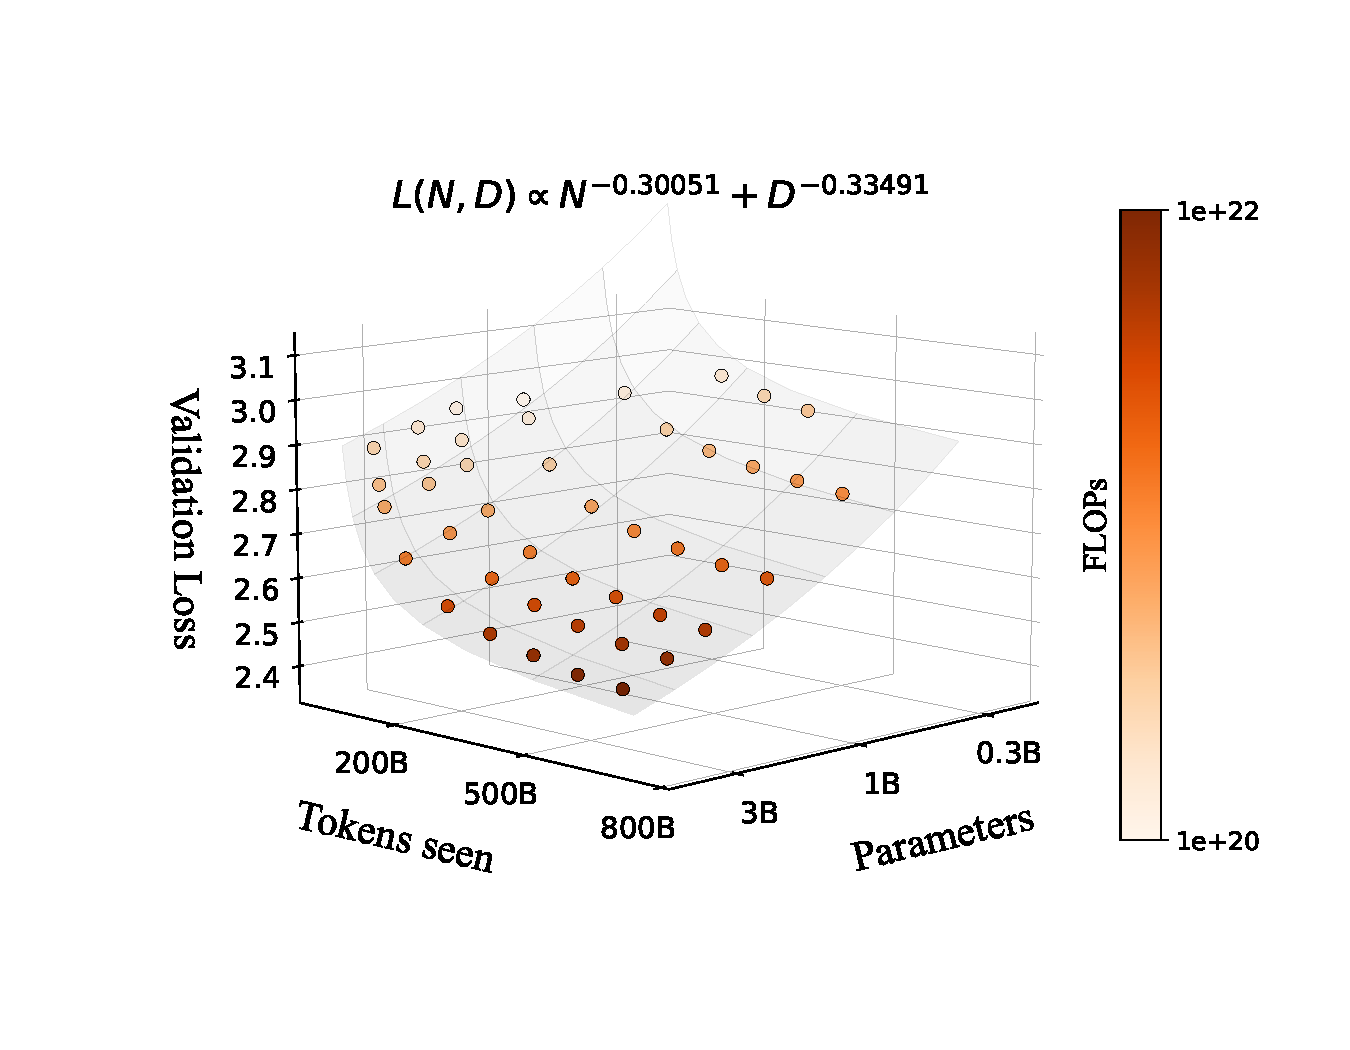
\includegraphics[width=1.02\linewidth]{assets/early/3d_scaling_early.pdf}
    \end{subfigure}
    \hfil
    \begin{subfigure}[t]{0.48\linewidth}
        \centering
        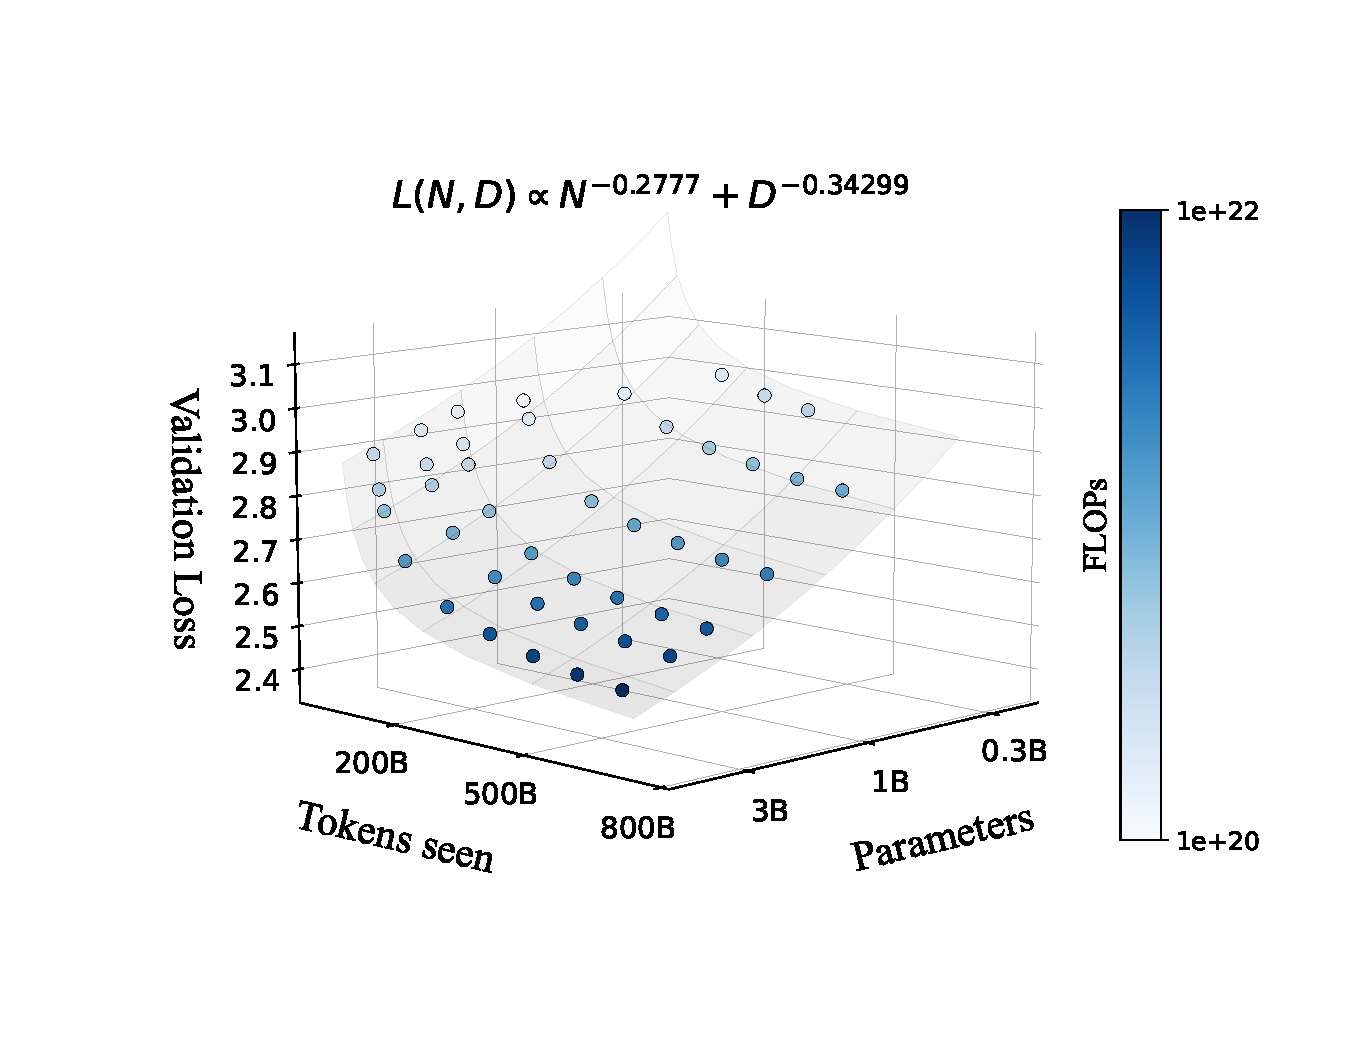
\includegraphics[width=1.02\linewidth]{assets/early/3d_scaling_late.pdf}
    \end{subfigure}
    \vspace{5pt}
    \setlength{\fboxsep}{0.5pt}
    \setlength{\fboxrule}{0pt}
    \caption{\textbf{原生多模态模型中 \fbox{\colorbox{CustomC_Light1!20}{\strut early-fusion}} 与 \fbox{\colorbox{CustomD_Light1!20}{late-fusion\strut}} 的尺度规律。} 每个点表示一个在不同 \edit{数量的} tokens(250M 到 400B)上训练的模型(300M 到 3B 参数)。我们报告了在 \edit{交错数据(Obelics)、图像描述数据(HQITP)和纯文本数据(DCLM)} 的验证集上的平均交叉熵损失。}
    \label{fig:early_vs_late_scaleflops_3d}
\end{figure}


\begin{table}[h]
    \centering
    \setlength{\tabcolsep}{16pt}
    \renewcommand{\arraystretch}{1}
    \resizebox{1\linewidth}{!}{
    \begin{tabular}{lccrc}
        Data type & dataset & \#samples & sampling prob. \\
         \shline
         \multirow{3}{*}{Image-Caption} &  DFN~\citep{fang2023data} & 2B & 27\%
         \\
          & COYO~{\citep{kakaobrain2022coyo700m}} &  600M & 11.25\% \\
          & HQITP  & 400M & 6.75\% \\
          Interleaved & Obelics \citep{laurenccon2024obelics}  & 141M Docs &
          45\% \\
          Text & DCLM \citep{li2024datacomp} & 6.6T Toks & 10\% \\

    \end{tabular}} \caption{\textbf{预训练数据混合。}除非另有说明,训练数据混合中包含 45\%、45\% 和 10\% 的图像标题、交错文档和纯文本数据。}
    \label{tab:pretraining_datasets}
    \vspace{-5pt}
\end{table}
\subsection{实验设置}
\edit{我们的模型} 基于自回归变换器架构~\citep{vaswani2017attention},使用SwiGLU FFN~\citep{shazeer2020glu} 和QK-Norm~\citep{dehghani2023scaling},遵循~\citet{li2024datacomp}。在早期融合模型中,图像块被线性映射以匹配文本标记维度,而后期融合遵循CLIP架构~\citep{radford2021learning}。我们对文本标记采用因果注意力,对图像标记采用双向注意力,发现这样效果更好。训练在公开和私人多模态数据集的混合上进行,包括DCLM \citep{li2024datacomp}、Obelics \citep{laurenccon2024obelics}、DFN \citep{fang2023data}、COYO \citep{kakaobrain2022coyo700m},以及一个私有的高质量图像-文本对(HQITP)集合(见\cref{tab:pretraining_datasets})。图像被\edit{调整大小}至224×224分辨率,图像块大小为14×14。我们使用1k的上下文长度来处理多模态序列。为了提高训练效率,我们使用\texttt{bfloat16}、完全分片数据并行(FSDP)\citep{zhao2023pytorch}、\edit{激活}检查点和梯度累积。我们还使用序列打包来处理图像标注数据集,以减少填充标记的数量。与之前的工作~\citep{hoffmann2022training,aghajanyan2023scalingmm,abnar2025parameters}类似,我们在交替的(Obelics)、图像-标注(HQITP)和仅文本数据(DCLM)上评估性能。更多的实现细节请参见~\cref{app:implementation_details}。
